\section{Abläufe}

Während in Kapitel 3 die Interaktion der Hauptkomponenten \emph{Server} und der \emph{RobotUnit} abgehandelt wurden, werden im Folgenden die Abläufe der Use Cases genauer spezifiziert und auch interne Komponentenabläufe beschrieben, im speziellen die Abläufe innerhalb der \emph{RobotUnit}.
	
	\subsection*{Interaktion bei Ausführung von Use Case 1 – \emph{DriveToDestination}}
	Wie schon der Name des Use Cases \emph{DriveToDestionation} beschreibt, befindet sich die \emph{RobotUnit} bei Ausführung diese Use Cases in einem Fahrvorgang, der vorher konkret mit der Zielposition und er Geschwindigkeit vom Server eingestellt wird. Es reagieren intern ihre Software mit den Sensor-/Hardwarekomponenten, wenn ein Hindernis auftaucht und dieses mit Hilfe der durch die Sensoren gesammelten Informationen umfahren werden muss. Der unmittelbare Fahrvorgang hingegen wird über die \emph{IDrive}-Schnittstelle gesteuert, die zurückmeldet, wenn der \emph{Robot} sein Ziel erreicht hat.
	
	Abbildung \ref{DriveToDestination} zeigt ein entsprechendes Sequenzdiagramm.
	
	\begin{figure}[H]
		\centering
		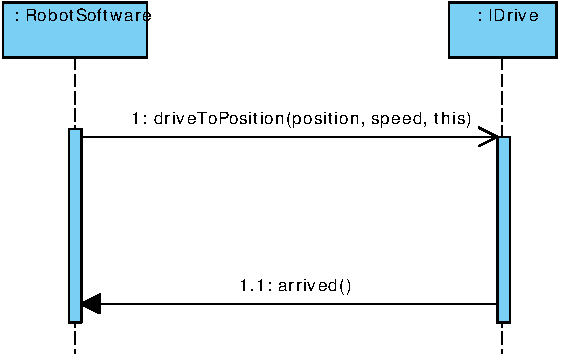
\includegraphics[width=0.75\textwidth]{img/8-driveToDest}
		\caption{Sequenzdiagramm von \emph{DriveToDestination}}
		\label{DriveToDestination}
	\end{figure}
	
	
	\subsection*{Interaktion bei Ausführung von Usecase 2 – \emph{ReadSensors}}
	In Abbildung \ref{ReadSensors} wird der reine Anfrageprozess zwischen \emph{Server} und der \emph{RobotUnit} aus Kapitel 3 erweitert. Nach der Anfrage wird der \emph{Robot} alle nötigen Informationen naheinander abfragen: Sowohl die \emph{Position} als auch die \emph{Orientation} werden von der \emph{INorthStar}-Schnittstelle zurückgeliefert. Für den Batteriestatus muss die \emph{IBattery}-Schnittstelle angefragt werden. Erst wenn alle Informationen als Gesamtpaket bereitstehen, können sie an den \emph{Server} zurückgemeldet werden.\\
	\begin{figure}[H]
		\centering
		\includegraphics[width=0.75\textwidth]{img/8-readSensors}
		\caption{Sequenzdiagramm von \emph{ReadSensors}}
		\label{ReadSensors}
	\end{figure}
	
	\subsection*{Interaktion bei Ausführung von Use Case 3 – \emph{Charging}}
	Auch beim Use Case \emph{Charging} findet keine Kommunikation mit der Komponente \emph{Server} statt, dafür allerdings zwischen der \emph{RobotUnit} und der \emph{ChargingStation}. Hat der \emph{Robot} einen bestimmten kritischen Ladestand erreicht (den er regelmäßig überprüft), steuert er die \emph{ChargingStation} an. Der Ladevorgang triggert automatisch, sobald der \emph{Robot} die \emph{Position} der Ladestation erreicht hat, und er interagiert so lange mit ihr, bis seine Batterie wieder aufgeladen ist. Innerhalb des \emph{Robots} werden zum Anfahren der \emph{ChargingStation} die Komponenten \emph{IBattery} mit der Position der robotereigenen Ladestation und \emph{IDrive} benötigt. Konkret: Wenn \emph{IDrive} \texttt{arrived()} zurückgibt, kann der Ladevorgang begonnen werden.
	
	Abbildung \ref{Charging} zeigt ein Sequenzdiagramm für den Use Case \textit{Charging}.
	
	\begin{figure}[H]
		\centering
		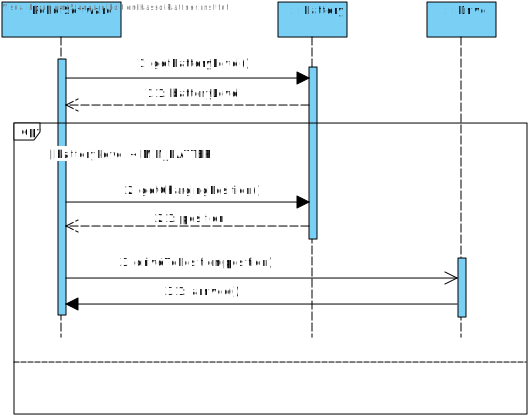
\includegraphics[width=0.75\textwidth]{img/8-charging}
		\caption{Sequenzdiagramm von \texttt{Charging}}
		\label{Charging}
	\end{figure}
